%%%%%%%%%%%%%%%%%%%%%%%%%%%%%%%%%%%%%%%%%
% baposter Landscape Poster
% LaTeX Template
% Version 1.0 (11/06/13)
%
% baposter Class Created by:
% Brian Amberg (baposter@brian-amberg.de)
%
% This template has been downloaded from:
% http://www.LaTeXTemplates.com
%
% License:
% CC BY-NC-SA 3.0 (http://creativecommons.org/licenses/by-nc-sa/3.0/)
%
%%%%%%%%%%%%%%%%%%%%%%%%%%%%%%%%%%%%%%%%%

%----------------------------------------------------------------------------------------
%	PACKAGES AND OTHER DOCUMENT CONFIGURATIONS
%----------------------------------------------------------------------------------------

\documentclass[landscape,a0paper,fontscale=0.285]{baposter} % Adjust the font scale/size here

\usepackage{graphicx} % Required for including images
\graphicspath{{figures/}} % Directory in which figures are stored

\usepackage{amsmath} % For typesetting math
\usepackage{amssymb} % Adds new symbols to be used in math mode

\usepackage{booktabs} % Top and bottom rules for tables
\usepackage{enumitem} % Used to reduce itemize/enumerate spacing
\usepackage{palatino} % Use the Palatino font
\usepackage[font=small,labelfont=bf]{caption} % Required for specifying captions to tables and figures

\usepackage{multicol} % Required for multiple columns
\setlength{\columnsep}{1.5em} % Slightly increase the space between columns
\setlength{\columnseprule}{0mm} % No horizontal rule between columns

\usepackage{tikz} % Required for flow chart
\usetikzlibrary{shapes,arrows} % Tikz libraries required for the flow chart in the template

\newcommand{\compresslist}{ % Define a command to reduce spacing within itemize/enumerate environments, this is used right after \begin{itemize} or \begin{enumerate}
\setlength{\itemsep}{1pt}
\setlength{\parskip}{0pt}
\setlength{\parsep}{0pt}
}

\definecolor{lightblue}{rgb}{0.145,0.6666,1} % Defines the color used for content box headers

\begin{document}

\begin{poster}
{
headerborder=closed, % Adds a border around the header of content boxes
colspacing=1em, % Column spacing
bgColorOne=white, % Background color for the gradient on the left side of the poster
bgColorTwo=white, % Background color for the gradient on the right side of the poster
borderColor=lightblue, % Border color
headerColorOne=black, % Background color for the header in the content boxes (left side)
headerColorTwo=lightblue, % Background color for the header in the content boxes (right side)
headerFontColor=white, % Text color for the header text in the content boxes
boxColorOne=white, % Background color of the content boxes
textborder=roundedleft, % Format of the border around content boxes, can be: none, bars, coils, triangles, rectangle, rounded, roundedsmall, roundedright or faded
eyecatcher=true, % Set to false for ignoring the left logo in the title and move the title left
headerheight=0.1\textheight, % Height of the header
headershape=roundedright, % Specify the rounded corner in the content box headers, can be: rectangle, small-rounded, roundedright, roundedleft or rounded
headerfont=\Large\bf\textsc, % Large, bold and sans serif font in the headers of content boxes
%textfont={\setlength{\parindent}{1.5em}}, % Uncomment for paragraph indentation
linewidth=2pt % Width of the border lines around content boxes
}
%----------------------------------------------------------------------------------------
%	TITLE SECTION 
%----------------------------------------------------------------------------------------
%
{
\includegraphics[height=4em]{logo.png}} % First university/lab logo on the left
{\bf\textsc{Ride Hailing Supply and Demand Forecasting using Didi-Tech Dataset}\vspace{0.5em}} % Poster title
{\textsc{\{ Gopal Menon and Kimberly Williamson \} \hspace{12pt} University of Utah Data Mining Spring 2017}} % Author names and institution

%----------------------------------------------------------------------------------------
%	Introduction
%----------------------------------------------------------------------------------------

\headerbox{Introduction}{name=objectives,column=0,span=2,row=0}{

Didi Chuxing is the leading ride hailing company in China and processes over 11 million trips, plans over 9 billion routes and collects over 50TB of data per day. They organized a worldwide algorithm challenge in the year 2016 [1] for forecasting ride supply and demand. We used the 2016 Didi algorithm competition dataset to try and forecast taxi trip supply and demand for any given date, time, and location using regression models covered in the Data Mining 2017 Spring semester at the School of Computing of the University of Utah.  Below is a sample of some methods used:

\begin{enumerate}\compresslist
\item Stochastic Gradient Descent
\item Polynomial Regression
\item Gaussian Kernel Regression
\item Hierarchial Clustering
\end{enumerate}

\vspace{0.3em} % When there are two boxes, some whitespace may need to be added if the one on the right has more content
}

%----------------------------------------------------------------------------------------
%	PATTERNS IN RIDE HAILING DATA
%----------------------------------------------------------------------------------------

\headerbox{Patterns In Ride Hailing Data}{name=results,column=2,span=2,row=0}{

\begin{multicols}{2}
\vspace{1em}
\begin{center}
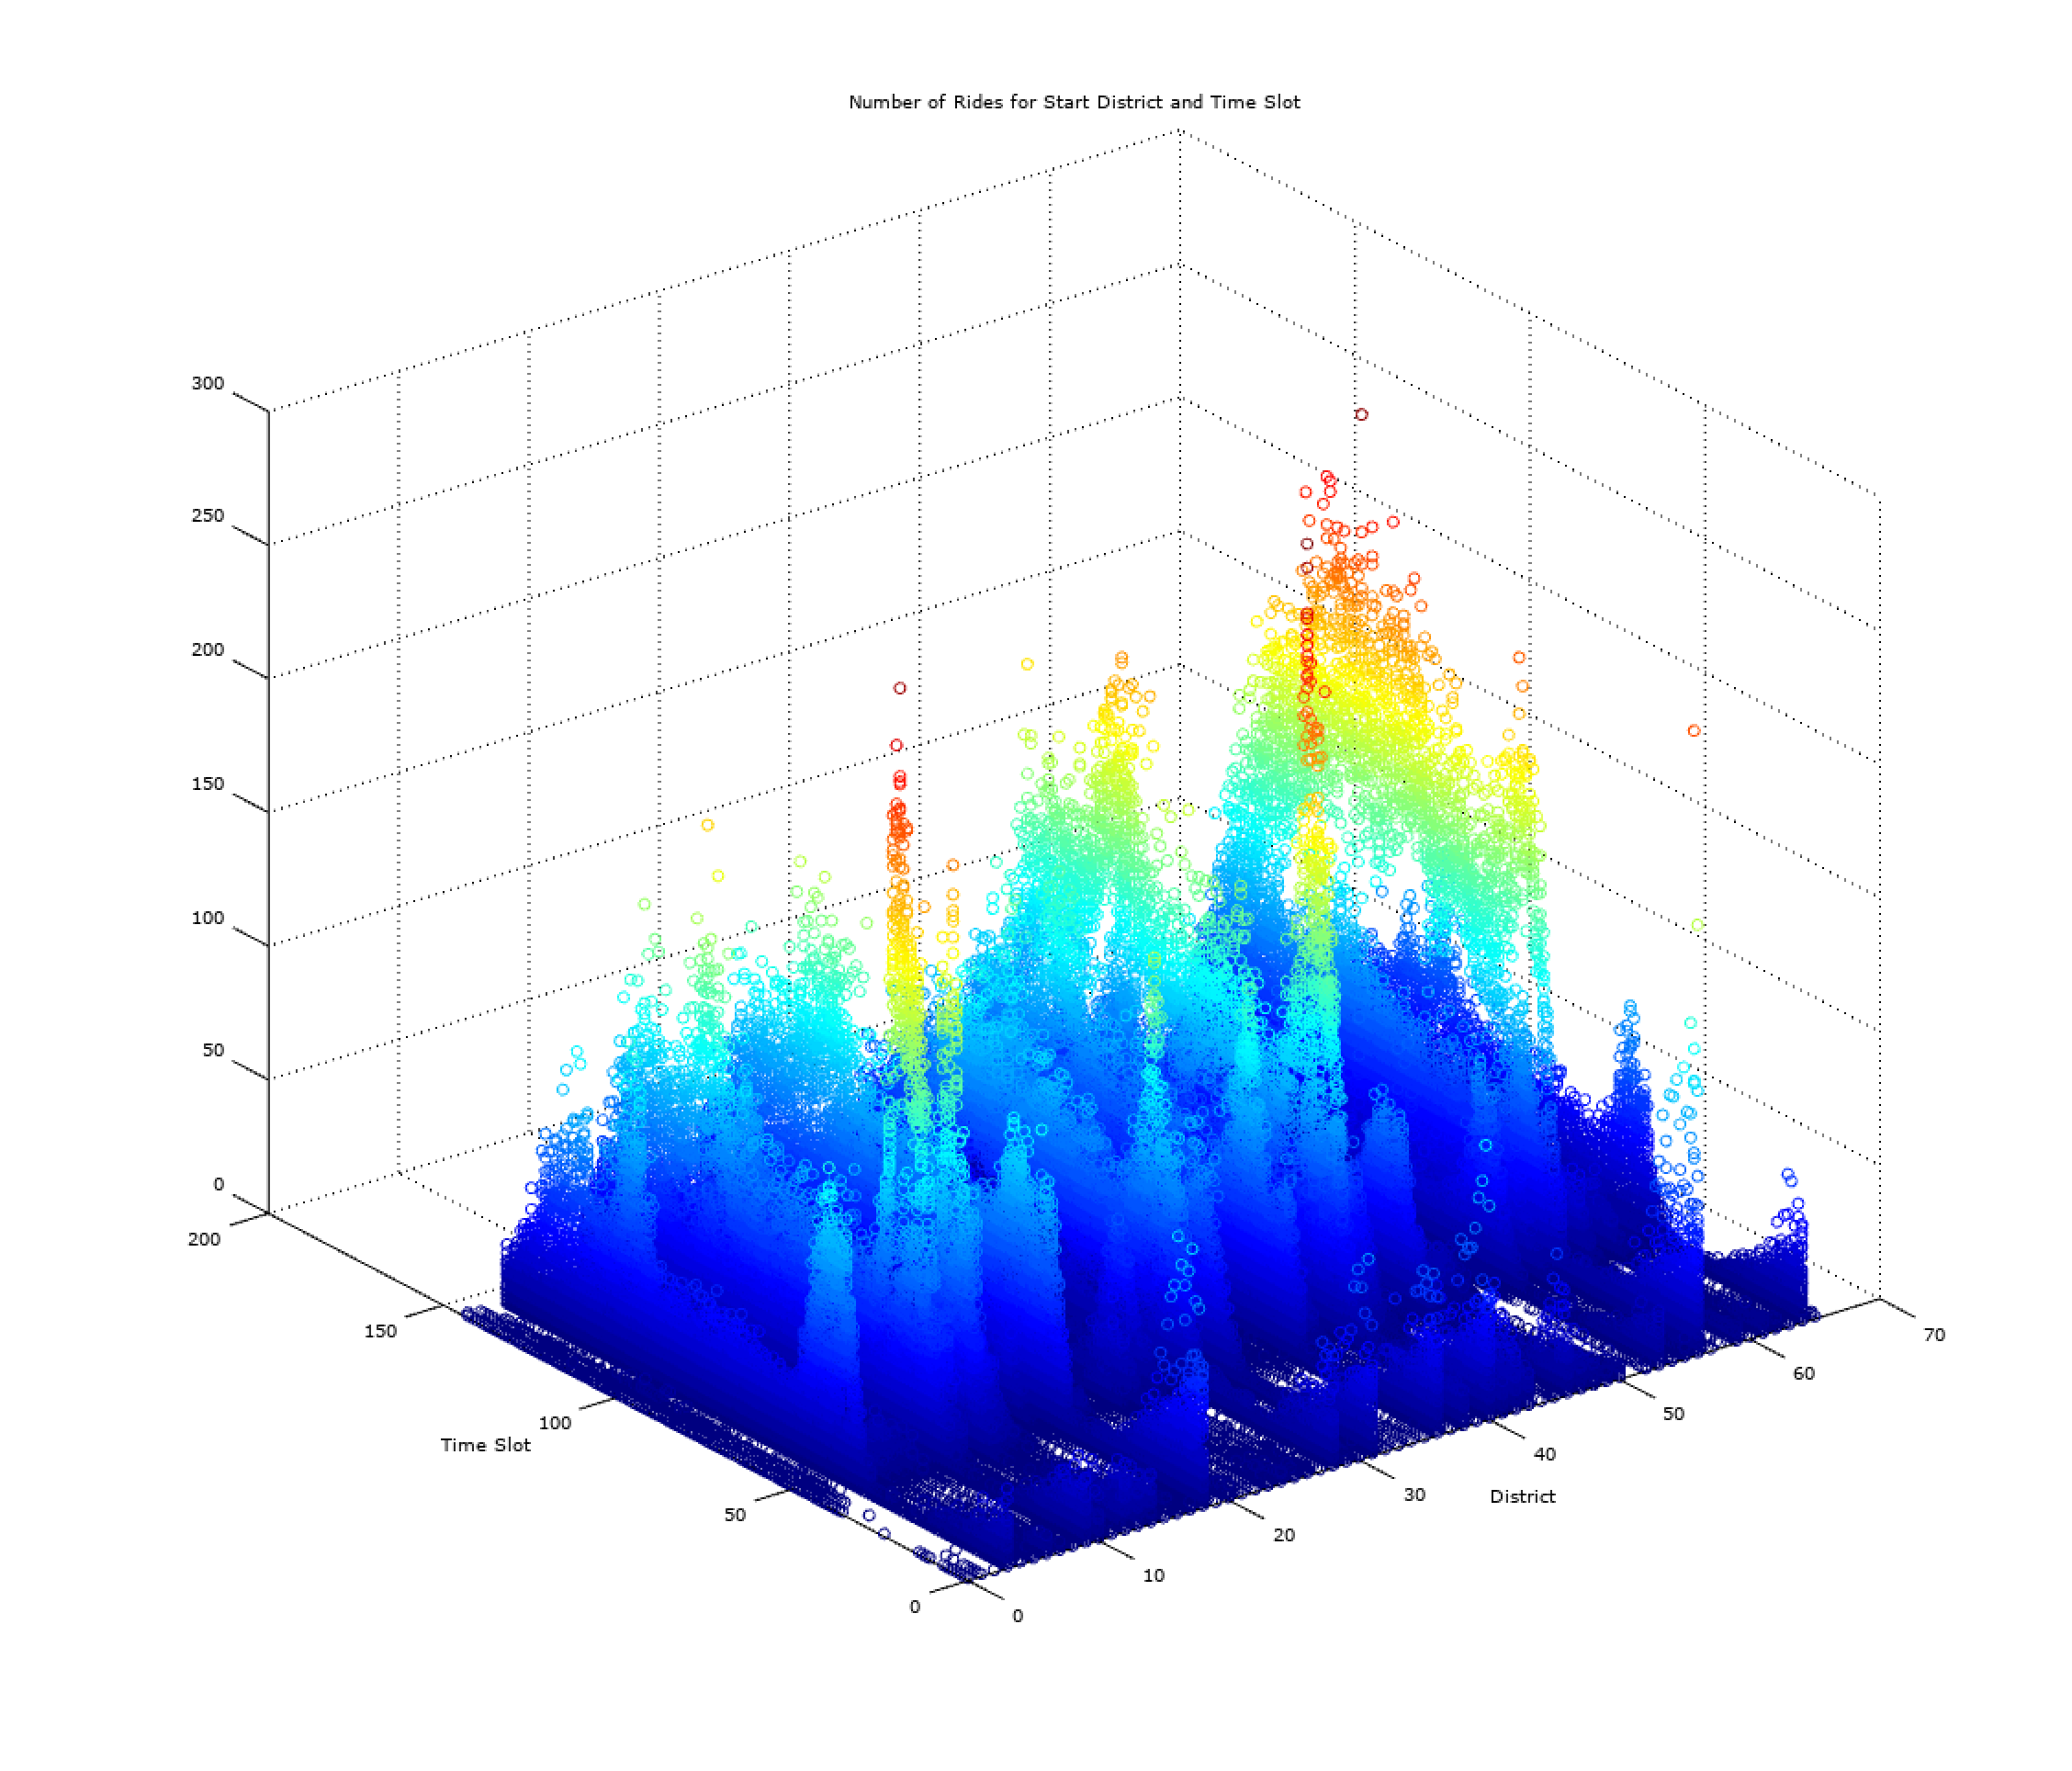
\includegraphics[width=0.8\linewidth]{figures/NumberofRidesforDistrictandTimeSlot.png}
\captionof{figure}{Number of rides scatter plot for start district and time slot.}
\end{center}

We also looked at patterns that could be attributed to the passengers taking taxis to and from work. Using a Monday through Friday work week, we first found the peak timeslots. Then using the peak timeslots, we plotted the number of orders per start district and the number of orders per destination district for the first peak. While there does appear to be some pattern that could lead to deducing residential and commercial districts, the pattern is not strong enough to reduce the complexity of the dataset.
\end{multicols}

%------------------------------------------------

\begin{multicols}{2}
\vspace{1em}
Since we were not getting good results, we decided to look for outliers. The outliers are usually computed using the inter-quartile distance between the first and third quartiles and using that value to include elements that are up to $1.5$ times the inter-quartile distance on either side. Elements outside these limits are marked as outliers. However it is doubtful that these are outliers since it is actual data and the reported number of outliers is large.  \\

We next looked at clustering methods to determine and filter out outliers. After experimenting with a couple of methods, there was no improvement in the mean squared error. We confirmed our previous theory that the identified outliers are most likely not true outliers, but result of the scattered nature of the dataset. \\

\begin{center}
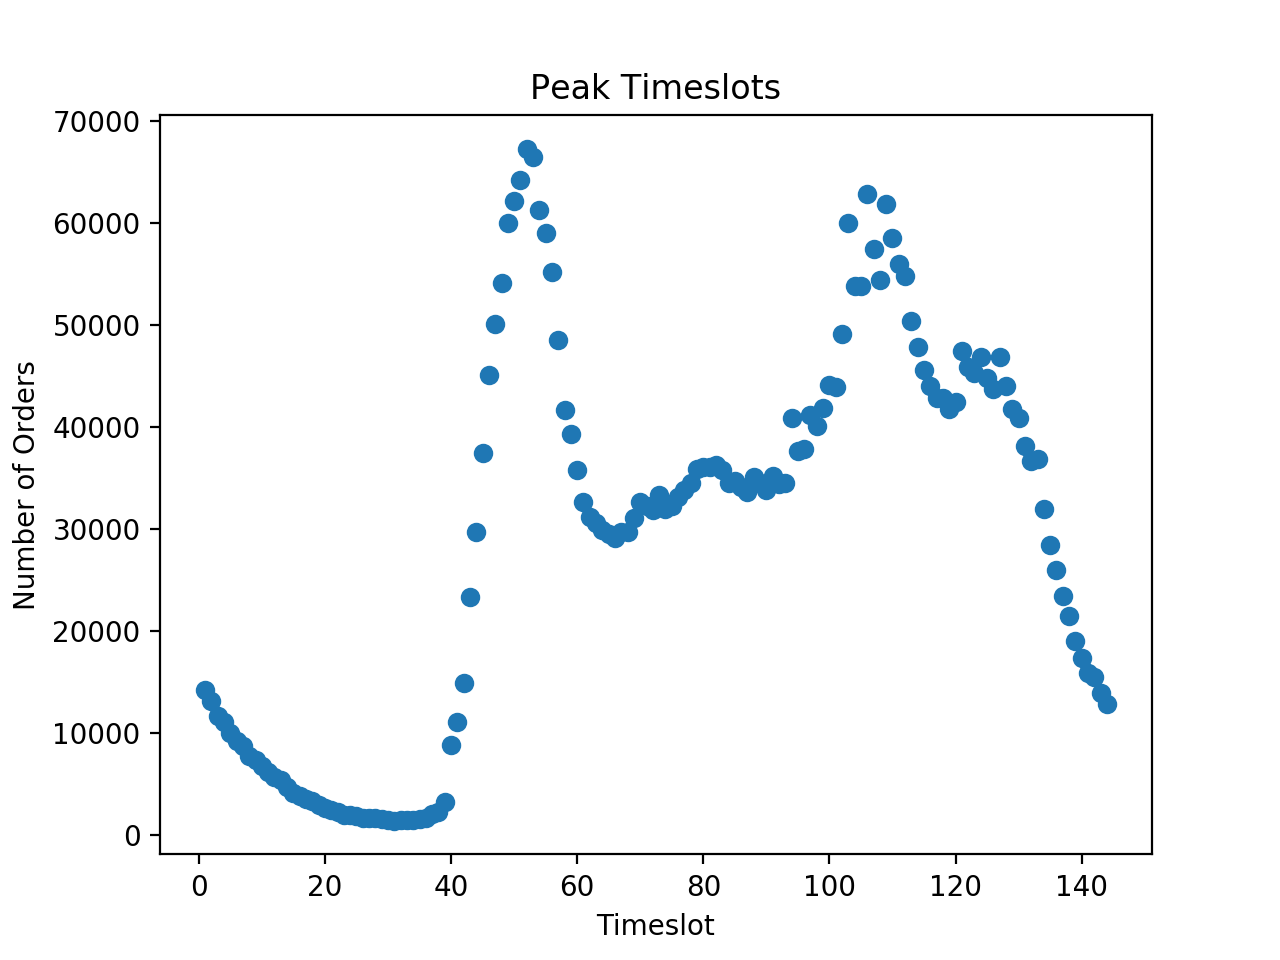
\includegraphics[width=0.8\linewidth]{figures/PeakTimeslots.png}
\captionof{figure}{Number of rides scatter plot for a timeslot (Monday-Friday).}
\end{center}

\end{multicols}
}

%----------------------------------------------------------------------------------------
%	REFERENCES
%----------------------------------------------------------------------------------------

\headerbox{References}{name=references,column=0,above=bottom}{

\renewcommand{\section}[2]{\vskip 0.05em} % Get rid of the default "References" section title
\nocite{*} % Insert publications even if they are not cited in the poster
\small{ % Reduce the font size in this block
\bibliographystyle{unsrt}
\bibliography{sample} % Use sample.bib as the bibliography file
}}


%----------------------------------------------------------------------------------------
%	CONCLUSION
%----------------------------------------------------------------------------------------

\headerbox{Conclusion}{name=conclusion,column=2,span=2,row=0,below=results,above=references}{

It looks like traditional regression methods do not work for complicated situations where we need to model human behavior. Deep learning techniques have been shown to give better results where traditional methods have failed or do not result in the desired level of accuracy. This is possibly a problem that is better suited to using deep learning.

}

%----------------------------------------------------------------------------------------
%	Ride Hailing Data
%----------------------------------------------------------------------------------------

\headerbox{Ride Hailing Data}{name=method,column=0,span=2,below=objectives}{ % This block's bottom aligns with the bottom of the conclusion block

In order to run the regression models, the categorical values in the Didi algorithm competition dataset needed to be converted into a regression friendly format. Depending on the type of categorical value, the new values are lists that consist of 0 values when the category is not present in an order and 1 or a count when the category is present in the order. \\

We have 1.3million rows in our training data consisting of ride hailing orders. When we took into consideration, only those orders where the start and end districts have data for traffic and places of interest, the number of training rows were reduced to 921,000.
}

%----------------------------------------------------------------------------------------
%	Regression Results
%----------------------------------------------------------------------------------------

\headerbox{Regression Results}{name=results2, column=0, span=2, below=method,bottomaligned=conclusion}{ % This block's bottom aligns with the bottom of the conclusion block

\begin{center}
    \begin{tabular}{|l|r|}
      \hline
   Regression Type  & Mean Squared Error \\
      \hline      
      Linear using Stochastic Gradient Descent&   $245.50$ \\
      \hline      
      Gradient Boosting using features based on top $10$ eigen vectors &    $285.97$    \\
      \hline
      Ridge Regression using features based on top $10$ eigen vectors&    $293.83$    \\
      \hline
      Lasso Regression using features based on top $10$ eigen vectors&    $293.83$    \\
      \hline
     Polynomial degree 2 regression using features based on top $10$ eigen vectors &    $2.34\times10^{53}$    \\
      \hline
     Polynomial degree 3 regression using features based on top $10$ eigen vectors &    $3.53\times10^{73}$    \\
      \hline
     Polynomial degree 4 regression using features based on top $10$ eigen vectors &    $9.31\times10^{93}$    \\
      \hline
      Gaussian Kernel Regression &    $376.90$    \\
      \hline
    \end{tabular}
	\captionof{table}{Table caption}
    \end{center}
}
%----------------------------------------------------------------------------------------

\end{poster}

\end{document}